\documentclass{beamer}

\usepackage[
backend=biber,
style=authoryear,
maxcitenames=3,
maxbibnames=3,
uniquelist=false,
backref=true,
doi=false,
isbn=false,
url=false,
eprint=false,
backref=false
]{biblatex}
\addbibresource{/Users/timbarry/optionFiles/tims_proposal.bib}

%Information to be included in the title page:
\title{Is \textit{BC} the new \textit{BH}?}
\subtitle{A tale of two multiple hypothesis testing procedures}
\author{Tim Barry}
\date{January 28, 2021}

\begin{document}

\frame{\titlepage}

\begin{frame}
\frametitle{Shifting my statistical focus}
\begin{itemize}
\item \textbf{Before}
\begin{itemize}
\item exponential families
\item measurement error models
\item latent variable models
\end{itemize}
\item \textbf{Now}
\begin{itemize}
\item \textcolor{blue}{multiple testing and false discovery rates}
\item conditional independence testing
\item negative control methods
\item robust inference
\end{itemize}
\end{itemize}
\end{frame}


\begin{frame}
\frametitle{Multiple testing review}
Consider $m$ hypothesis $H_1, \dots, H_m$. Suppose that we test these hypotheses and make $R$ discoveries. Of these discoveries, suppose that $V$ are \textit{false} discoveries (i.e., true nulls) and that $V - R$ are \textit{true discoveries} (i.e., true alternatives).

\begin{figure}
	\centering
	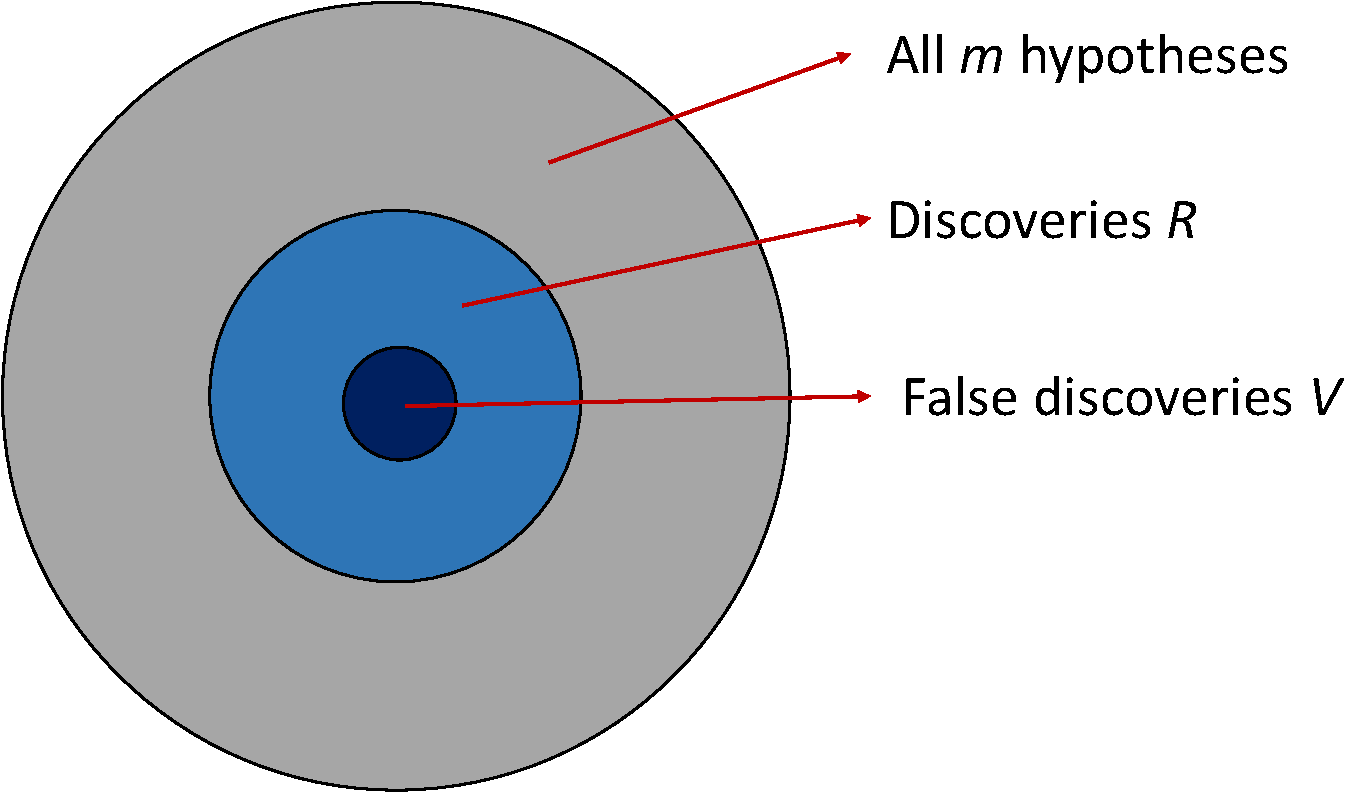
\includegraphics[width=0.8\linewidth]{fdr_fig}
	\label{fdrfig}
\end{figure}
\end{frame}

\begin{frame}
\frametitle{Multiple testing review: FDR and FWER}
The family-wise error rate (FWER) is the probability of making even $1$ false discovery:
$$FWER = \mathbb{P}(V \geq 1).$$
The false discovery rate (FDR) is the expected fraction of false discoveries:
$$FDR = \mathbb{E}\left( \frac{V}{ \max\{ R, 1 \}} \right) := \mathbb{E} \left( FDP \right).$$
If $R = 0$ (i.e., no discoveries), then
$$ FDR = 0.$$
\end{frame}

\begin{frame}
\frametitle{Benjamini-Hochberg (BH)}
\textbf{BH Procedure}: Suppose that we calculate $p$-values $p_1, \dots, p_m$ for the hypotheses $H_1, \dots, H_m$. Suppose that the $p$-values corresponding to the true null hypotheses are $U(0,1)$, and suppose that the $p_i$s are independent. Let $p_{(1)} \leq \dots, \leq p_{(m)}$ be the ordered $p$-values and $H_{(1)}, \dots, H_{(m)}$ the corresponding ordered hypotheses. Let $\alpha \in (0,1)$ be the user-chosen FDR level (typically, $\alpha \in \{ 0.05, 0.1, 0.2\}$). Define
$$\hat{k} = \textrm{argmax}_{k} \{ p_{(k)} \leq \alpha k /m \}.$$
Reject $H_{(1)}, \dots, H_{(\hat{k})}$.

\textbf{Theorem}: The BH procedure controls the FDR at level $\alpha$, i.e. $FDR \leq \alpha.$

\end{frame}

\begin{frame}
\frametitle{Visual interpretation of BH}

\begin{figure}
	\centering
	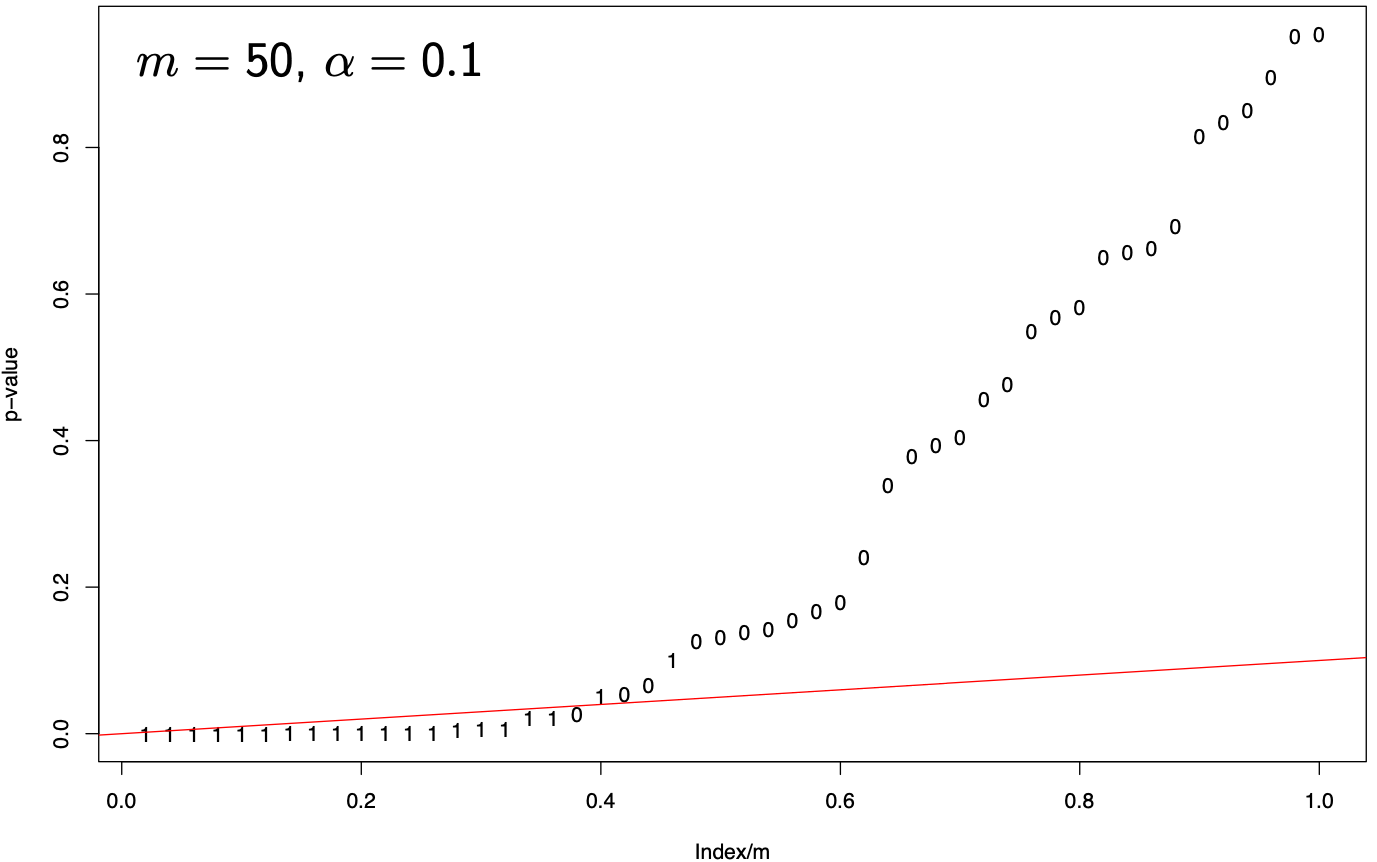
\includegraphics[width=1\linewidth]{bh_fig}
	\label{bhfig}
\end{figure}
(source: Chris Genovese)
\end{frame}

\begin{frame}
\frametitle{The Barber-Cand\'es (BC) procedure}
\textbf{BC procedure}  \parencite{Barber2015} : Let $X_1, \dots X_m$ be test statistics corresponding to the hypotheses $H_1, \dots, H_m$, with large values indicating evidence against the null hypothesis. Assume that the density $\psi$ of the null test statistics is symmetric about $0$, i.e. $\psi( x ) = \psi( -x )$ for all $x \geq 0$. Also, assume that the $X_i$s are independent. Let $|X| := \{ |X_i| : i = 1, \dots, n \}$ be the set of sample absolute values, and let $$\widehat{FPD}(t) := \frac{ 1 + \# \{ i:X_i \leq -t \} }{ \textrm{max} \left( 1, \# \{ i  : X_i \geq t \} \right) }$$ be the empirical false discovery proportion for given $t \in |X|.$ Finally, let $\alpha \in (0,1)$ be the FDR target. The BC threshold is $\tau_{\textrm{BC}} = \min \left\{ t \in |X| : \widehat{FDP}(t) \leq \alpha \right\}.$ Reject all $X_i \geq \tau_{\textrm{BC}}$.

\textbf{Theorem}: The BC procedure controls FDR at level $\alpha$, i.e. $FDR \leq \alpha$.
\end{frame}

\begin{frame}
\frametitle{BC procedure note}
\textbf{Note}: The null $X_i$s are \textbf{not} $p$-values. Instead, the null $X_i$s are test statistics with a shared, symmetric density. For example:
\begin{itemize}
\item Gaussian
\item Double exponential (AKA Laplace)
\item Student's $t$
\item Rademacher
\item Unknown symmetric distribution
\item etc.
\end{itemize}
\textbf{Tim's thought}: We can run BC on transformed $p$-values. Let $p_i \sim \textrm{U}(0,1)$ be a null $p$-value. For $c > 0$, let $X_i := c(-p_i + 1/2).$ Then $X_i \sim \textrm{U}(-c, c)$, with large values indicating evidence against the null. \textbf{Therefore, BC is more flexible than BH.}
\end{frame}

\begin{frame}
\frametitle{Visual interpretation of BC}
\begin{itemize}
\item Let $X_1, \dots, X_{10,000} \sim N(0,1)$ be the test statistics under the null hypothesis. Let $Y_1, \dots, Y_{500} \sim N(3.5, 1)$ be the test statistics under the alternative hypothesis. Let $$ Z := [X_1, \dots, X_{10,000}, Y_1, \dots, Y_{500}]$$ be the full vector of test statistics. 
\item We apply BC to $Z$ with the goal of discovering the $Y_i$s with FDR control at level $0.1$.
\end{itemize}
\end{frame}

\begin{frame}
\frametitle{Visual interpretation of BC}
\begin{figure}
	\centering
	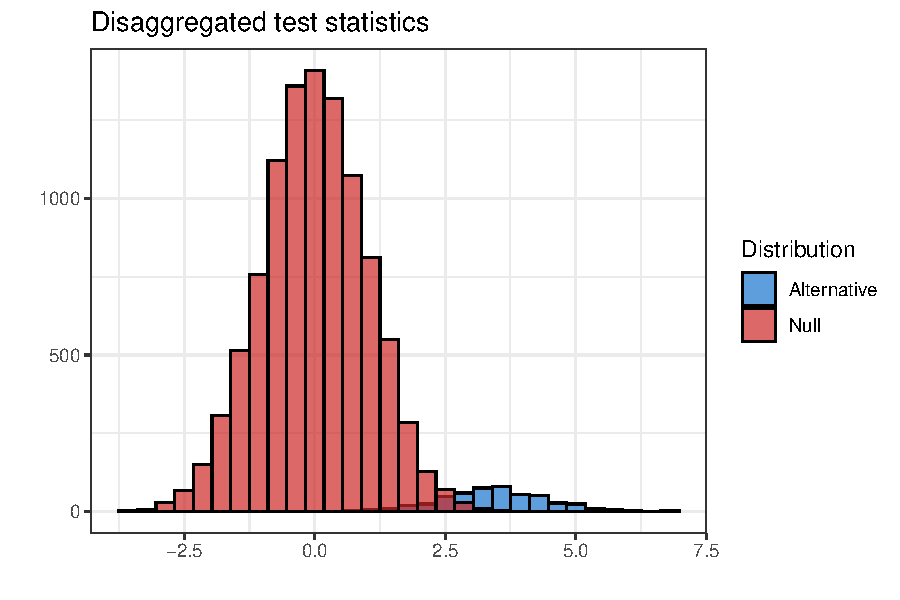
\includegraphics[width=1\linewidth]{disag_test_stats}
\end{figure}
\end{frame}

\begin{frame}
\frametitle{Visual interpretation of BC}
The \textcolor{blue}{blue}, \textcolor{red}{red}, and \textcolor{green}{green} vertical lines represent different candidate thresholds (at \textcolor{blue}{4.5}, \textcolor{red}{3.5}, and \textcolor{green}{2.65}, respectively).
\begin{figure}
	\centering
	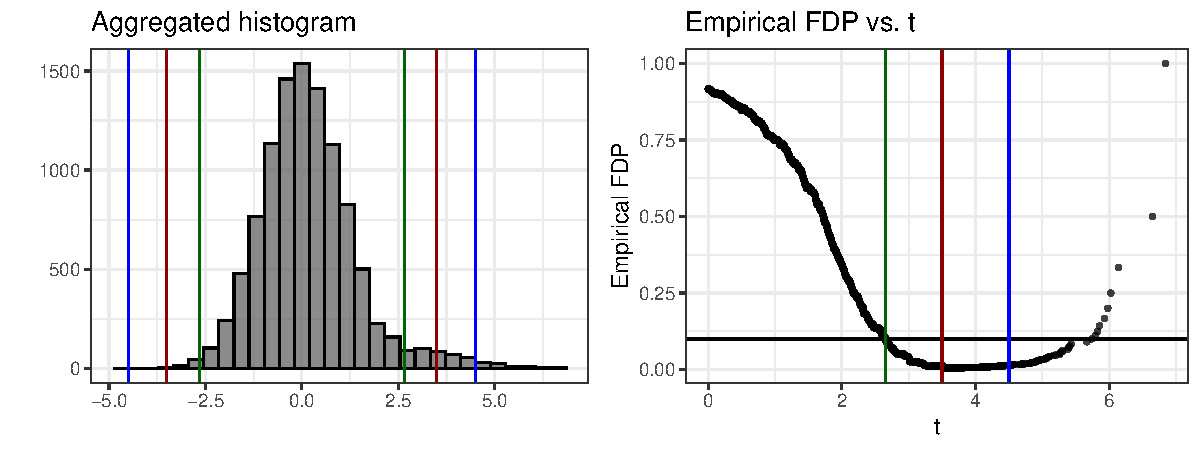
\includegraphics[width=1.0\linewidth]{agg_test_stats}
\end{figure}
The BC threshold is at \textcolor{green}{2.65}; thus, we reject all test statistics greater than this value.
\end{frame}

\begin{frame}
\frametitle{Power}

\begin{itemize}
\item Let $S$ be the number of \textit{true alternatives}, and let $Q$ be the number of \textit{non-discovered} true alternatives. The \textit{false non-discovery rate} ($FNR$) is 
$$FNR := \mathbb{E} \left[ \frac{Q}{ \max\{ S, 1 \} } \right].$$
\item FDR is analogous to type I error; FNR is analogous to type II error.

\end{itemize}
\begin{figure}
	\centering
	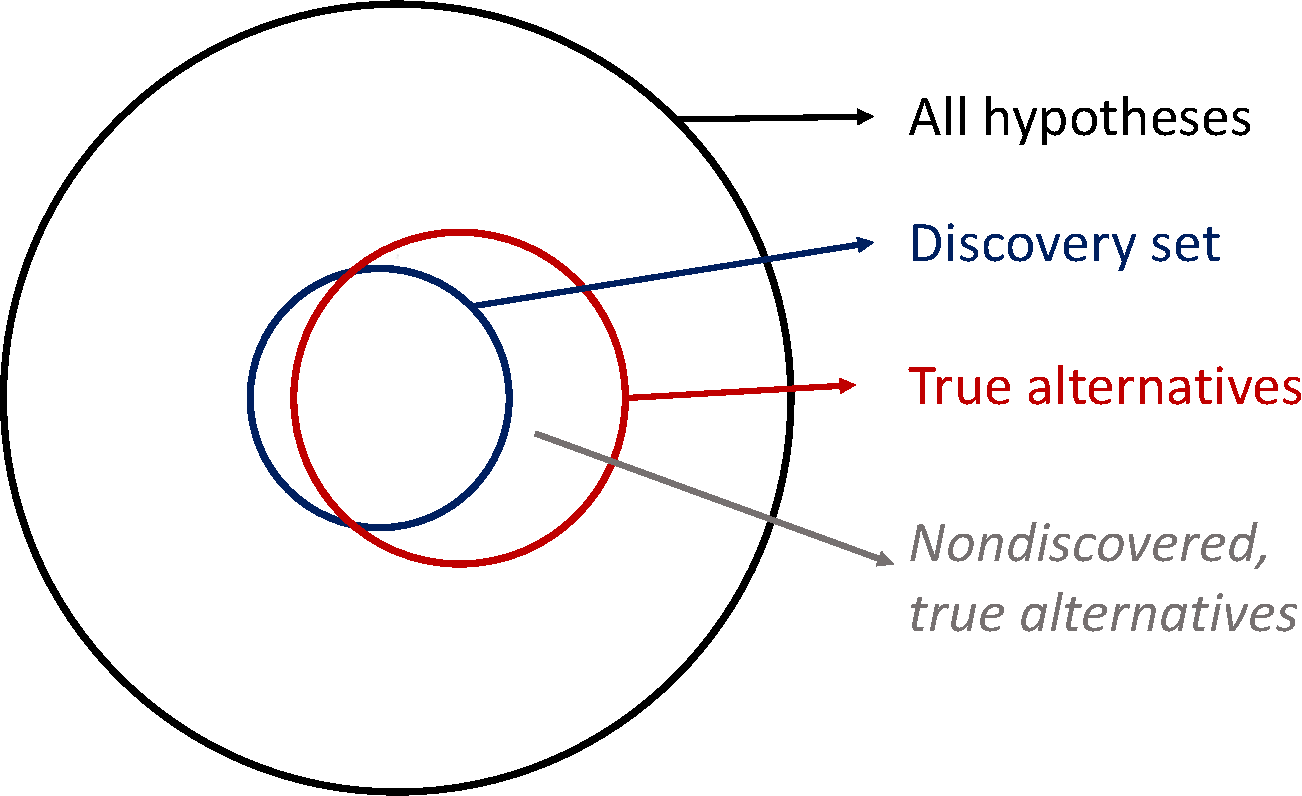
\includegraphics[width=0.6\linewidth]{fnr_crop}
	\label{fig:fnrcrop}
\end{figure}
\end{frame}

\begin{frame}
\frametitle{Power: numerical experiment}
I ran a small simulation experiment ($B = 50$ replicates) to compare the FDR (target: $< 10\%$) and FNR (smaller is better) of BC and BH in the example above. The results were similar across methods.

\begin{figure}
	\centering
	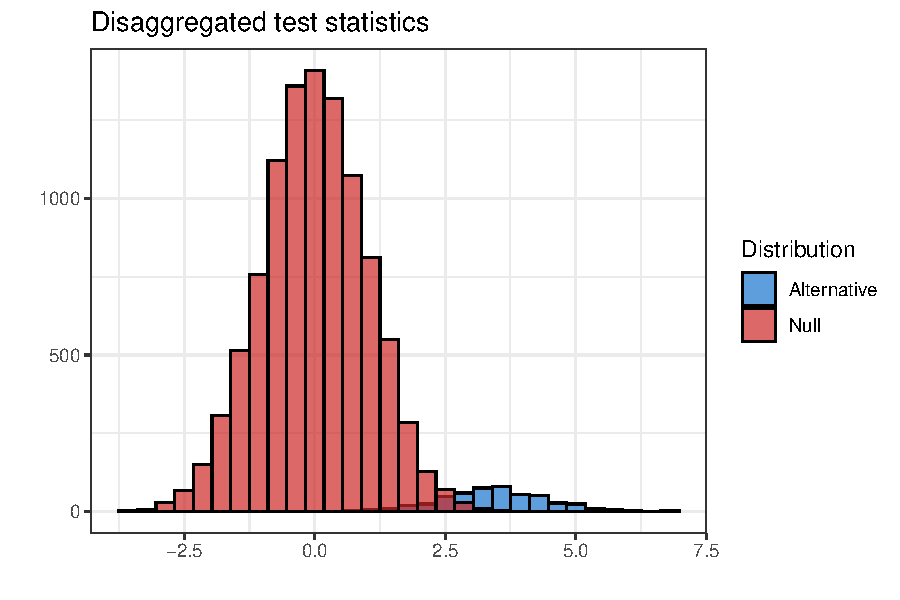
\includegraphics[width=0.5\linewidth]{disag_test_stats}
\end{figure}

\centering
\begin{tabular}{|c|c|c|}
	\hline 
	& BH & BC \\ 
	\hline 
	FDR & 9.7 \% & 9.8 \% \\ 
	\hline 
	FNR & 19.1 \% & 19.2 \% \\ 
	\hline 
\end{tabular} 
\end{frame}

\begin{frame}
\frametitle{Power: theoretical result}
\begin{itemize}
\item \textcite{Arias-Castro2017} showed that BC and BH have asymptotically identical power when the test statistics are Gaussian (as above).
\item The empirical experiments of \textcite{Arias-Castro2017} confirm their theoretical results. However, BC empirically seems lose power in ``ultrasparse'' (i.e., $< 1/1000$ hypotheses true) settings. More investigation is required.
\end{itemize}
\end{frame}

\begin{frame}
\frametitle{BC opens the door to new strategies for high-dimensional, robust, and/or nonparametric FDR control.}

\begin{itemize}
\item[1.] High-dimensional, nonparametric two-sample testing \parencite{Ge2021}.
\item[2.] Signal recovery in the (possibly high-dimensional) linear model \parencite{Barber2015}.
\item[2.] Doubly-robust, finite-sample calibration with negative controls (us 2022+?).
\end{itemize}
\end{frame}



\printbibliography
\end{document}

% BC opens the door to new, robust and/or nonparametric methods for FDR control.
